\chapter{Einleitung}

In den letzten Jahrzehnten konnten sich einige private Unternehmen erfolgreich in der Raumfahrt etablieren. Hierbei wird diese New Space Szene hauptsächlich von großen US-Firmen wie SpaceX, Virgin Galactic, Blue Origin dominiert, um nur ein paar zu nennen. Viele mehr versuchen auch noch weiterhin in dieser sich rasant entwickelnden Branche Fuß zu fassen. Bei so viel Konkurrenz sind Kosten ein wichtiger Faktor. Firmen wie SpaceX versuchen möglichst wirtschaftlich zu werden, indem sie immer größere Raketen bauen, die höhere Lasten auf einmal ins Weltall bringen können. So soll das Starship mehr als 100t in den Low Earth Orbit (LEO) bringen können. Das bringt aber auch einige Nachteile mit sich. Ein Start so großer Raketen ist nur mir sehr viel Beladung wirtschaftlich. So müssen sich mehrere Kunden einen Start teilen und sind somit sowohl in Bezug auf die Umlaufbahn als auch den Starttermin eingeschränkt. Gerade für einzelne, kleinere Satelliten ist das nicht ideal. Dies führt zur Ergründung eines weiten Bereiches der New Space Branche, den Microlaunchern. Mit ihren relativ kleinen Nutzlasten bieten sie die Möglichkeit flexibel die individuellen Ansprüche kleiner Satelliten, sogenannter CubeSats, zu berücksichtigen.

Ein weiteres Potenzial die Kosten zu senken bietet die Bergung und Wiederverwendung von Raketenstufen und Nutzlastverkleidung. Auch wenn sich ältere Projekte, wie das Space Shuttle, als nicht rentabel herausgestellt haben, können neuere Konzepte mehr Erfolge verbuchen. Ein modernes Beispiel bieten die erste Stufe der Falcon 9 oder auch die Booster der Falcon Heavy von SpaceX. Nach einem Reentry Burn, um bei dem Wiedereintritt in die Atmosphäre nicht zerstört zu werden, und eine Flugphase in der die Raketensegmente aerodynamisch zu einem Landeplatz gesteuert werden, kommt es zu einer erneuten Zündung der Triebwerke. Dadurch wird die Geschwindigkeit weit genug abgebremst, dass ein unversehrtes Aufsetzten möglich ist\cite{falconUserGuide}.
Rocket Lab verfolgt einen anderen Einsatz. Bei ihrer Electron Rakete soll die erste Stufe erst mit einem Ballute in den Unterschall und dann mit einem konventionellen Fallschirm weiter abgebremst werden. Dann kann diese entweder aus dem Wasser geborgen oder sogar direkt in der Luft von einem Hubschrauber eingefangen werden\cite{electronRocketLab}. Auch wenn diese Methode auf Grund des Bedarfs einer dichten Atmosphäre nur auf der Erde Anwendung findet und nur vergleichsweise kleine Raketenstufen von einem Hubschrauber getragen werden können, ist sie dank einer leichten Implementierung für simple Systeme vorzuziehen, da sie der komplizierte Teil, die aktive Landung, wegfällt.

Nun stellt sich die Frage, warum Europa und somit auch Deutschland, als eigentlich technologisch fortgeschrittener Standort, in dieser Branche nur spärlich vertreten ist. Ein großes Problem stellt hier die Wetterlage dar. Gerade im Norden Europas gehören Gewitter das ganze Jahr über zum Alltag und besonders im Herbst und Winter kann starker Wind und schwerer Schneefall potenziellen Starts im Wege stehen. Das begrenzt stark die Kapazität von Spaceports. Ein weiterer Nachteil des Standorts Europa ist die hohe Bevölkerungsdichte. Gerade im Westen ist somit kaum ein Start möglich, der genug Abstand zu besiedeltem Gebiet hält. Wegen der Erdrotation wird nach Osten gestartet, sodass auch Starts an der Küste zum Atlantik keine gute Option bieten.

\begin{figure}[h]
	\centering
	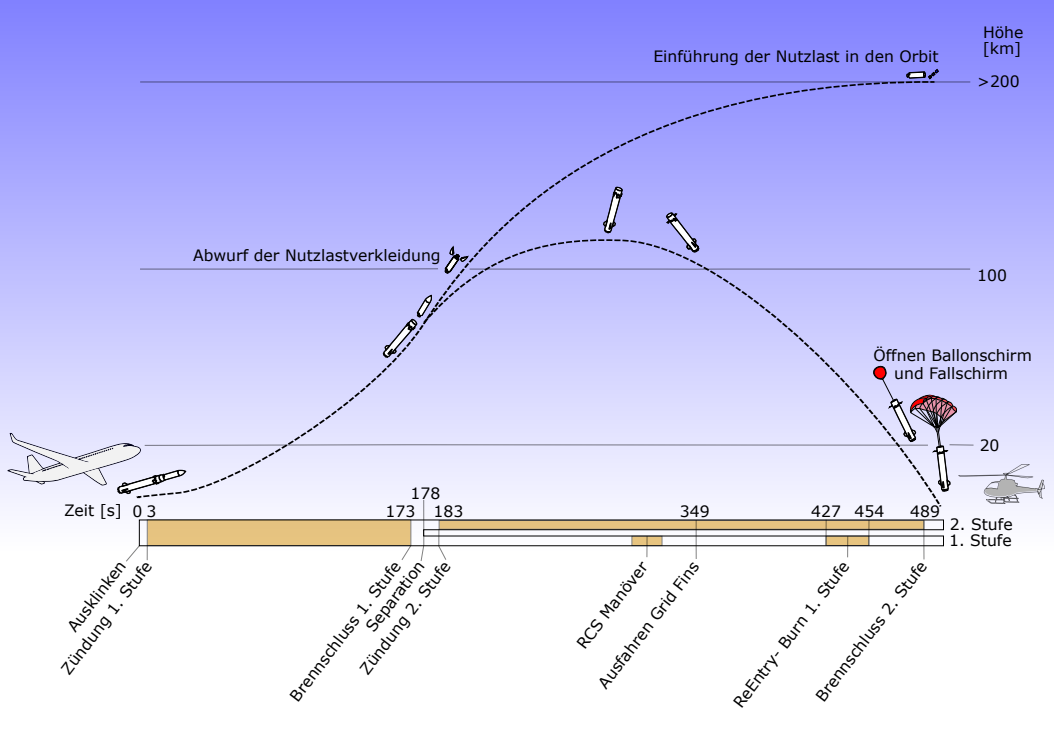
\includegraphics[width=\textwidth]{ablauf_valkyrie.png}
	\caption{Ablauf einer Valkyrie-Mission\cite{flugbahnBarz}}
\end{figure}

Als Antwort auf diese Probleme entwickelt die German Association for Intercontinental Astronautics e.V. (GAIA Aerospace) das Valkyrie System. Hierbei handelt es sich um eine zweistufige AirLaunch-Trägerrakete, die als Microlauncher kleine CubeSat aus Deutschland heraus in den LEO bringen soll\cite{GAIA}. Mit AirLaunch werden Raketen betitelt, die im Gegensatz zu klassischen Systemen nicht vertikal von der Erdoberfläche starten, sondern an einem Flugzeug befestigt in höhere Luftschichten gebracht werden und dort nach dem ausklinken aus der Halterung erst die Triebwerke zünden. Somit lässt sich sowohl das Problem des besiedelten Gebietes, indem die Trägerrakete zum Beispiel über die Nordsee gebracht wird, als auch die meisten störenden Wetterbedingungen umgehen. Die Valkyrie wird auf eine Höhe von 11 Kilometern gebracht\cite{flugbahnBarz} und ist somit über dem Wettergeschehen der Troposphäre. Eine hohe Wirtschaftlichkeit soll durch eine wiederverwendbare Erststufe gewährleistet werden. Beim Wiedereintritt soll sich diese, zusätzlich zu einer aerodynamischen Flugphase wie bei der Falcon 9, wie die Electron soweit in den Unterschall abbremsen, dass sich ein Fallschirm öffnen kann. Somit ist es dann möglich, dass ein Hubschrauber die Raketenstufe aus der Luft heraus auffängt und sicher an Land bringt.

\section{Motivation}
Für eine erfolgreiche Bergung der Erststufe der Valkyrie ist die aerodynamische Steuerung während der Flugphase von großer Bedeutung. So kann das Raketensegment sicher dorthin gelenkt werden, wo der Helikopter sie auch rechtzeitig erreichen kann, bevor diese ins Wasser fällt. Statische Stabilität im Flug herrscht immer dann, wenn der Druckpunkt hinter dem Schwerpunkt des Flugobjekts liegt. Beim Start sorgen hierfür vier Finnen am unteren Ende der Rakete. Im Apogäum führt die Erststufe eine 180°-Drehung um die eigene Achse durch, sodass die Triebwerke nach vorne zeigen. Dadurch haben nun die Finnen einen negativen Effekt auf die Stabilität und versuchen die Raketenstufe wieder zurück zu drehen. Um den entgegen zu wirken sollen am oberen Ende zusätzlich ein weiteres Quartett an Steuerflächen angebracht werden. Damit diese beim Start nicht ebenso eine negative Wirkung zeigen, soll hier ausklappbare Grid Fins (dt. Gitterflossen) verwendet werden.

\begin{figure}[h]
	\centering
	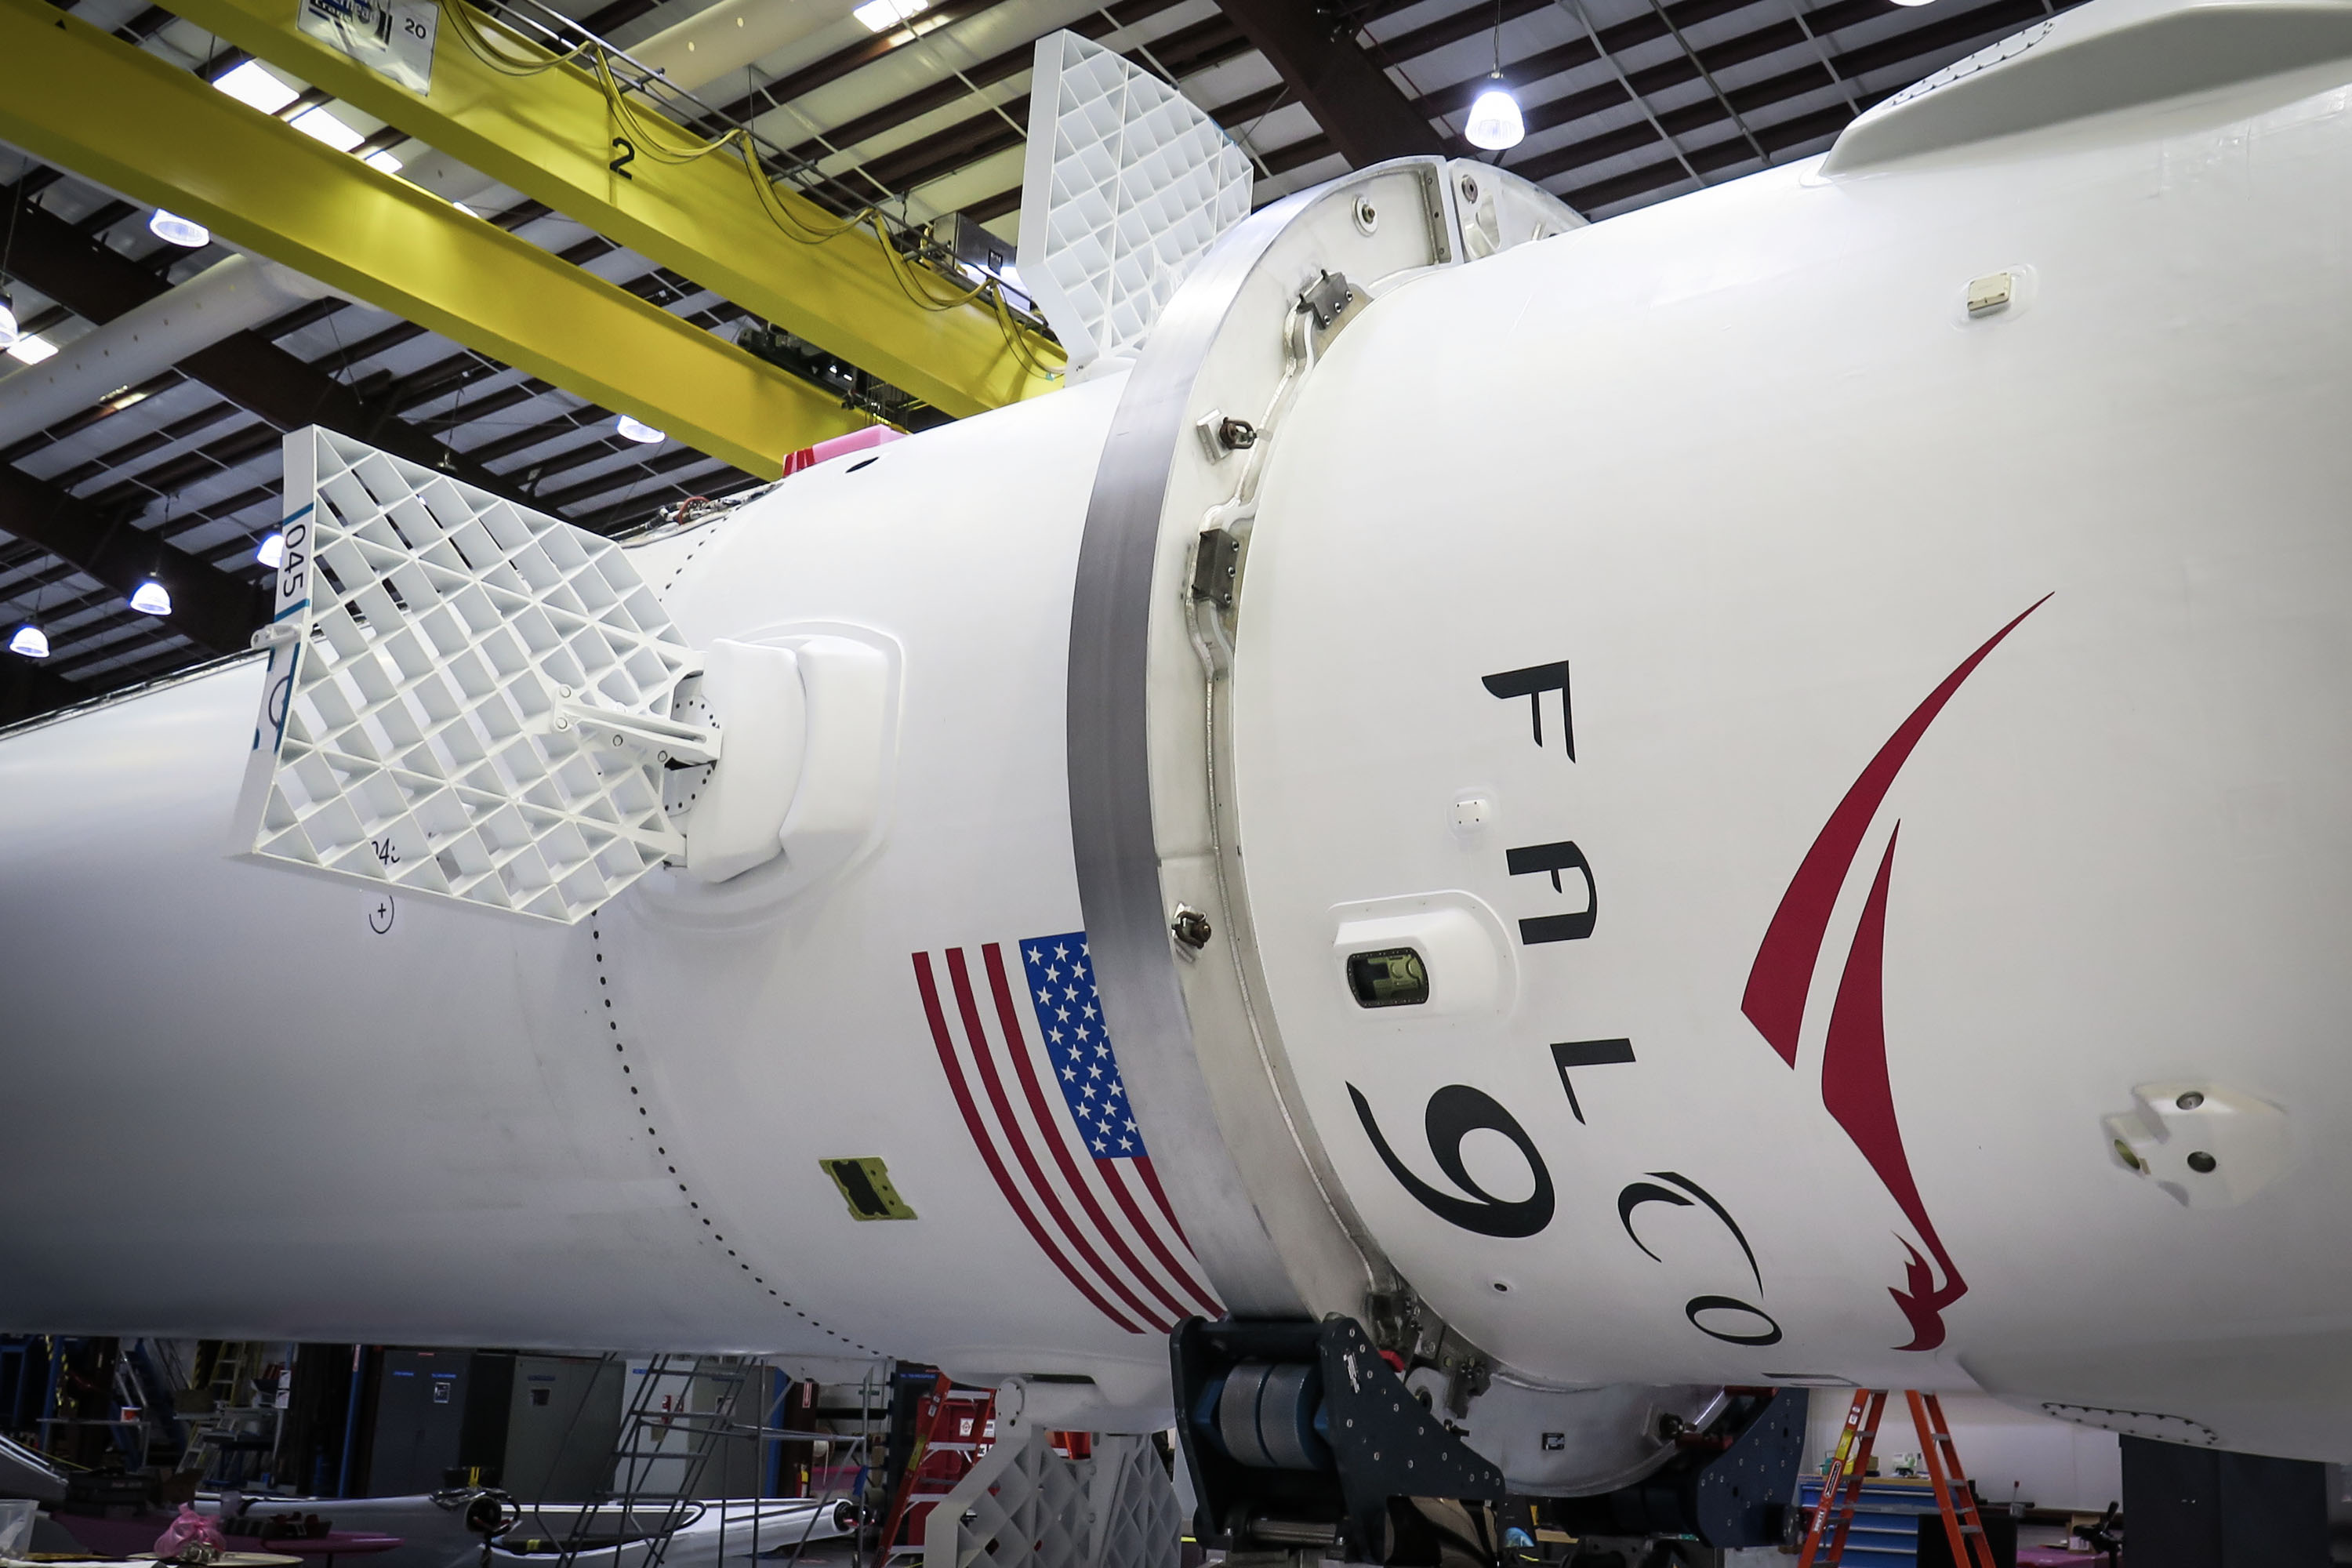
\includegraphics[width=0.8\textwidth]{fins_extended.jpg}
	\caption{Grid Fins am CRS-5 Falcon 9 Booster, Quelle: SpaceX}
\end{figure}

Grid Fins sind unkonventionelle Steuerelemente, die im Gegensatz zu ihrem planaren Gegenstück nicht parallel zur Strömung, sondern senkrecht dazu ausgerichtet sind. Sie bestehen aus einem dünnen äußeren Rahmen mit einer inneren Gitterstruktur. Die Möglichkeit sie einzuklappen hilft hier nicht nur ihre unerwünschte Wirkung bei Start zu umgehen, sondern erlaubt auch einen einfacheren Transport, wie zum Beispiel am Bug eines Flugzeuges. Ein geringes Moment um das Steuergelenk, so wie gute Auftriebserzeugung über einen großen Bereich von Anstellwinkeln und Machzahlen\cite{vergleichPlanar}, machen Grid Fins zu attraktiven Steuerelementen von Flugkörpern bei hohen Machzahlen.

Seit ihrer Entwicklung in den späten 50er-Jahren in der ehemaligen Sowjetunion, wurden sie in vielen ballistischen Raketen, wie zum Beispiel die Adder AA-12, SS-12 oder auch von der USA bei der Massive Ordiance Air Blast (MOAB) verwendet. Einen großen Nachteil der Grid Fins, ihren hohen Widerstand, hat sich das Launch Escape Vehicle der Soyuz zu Nutze gemacht, indem sie als Drag Breaks genutzt werden. Auch SpaceX bedient sich dieser Technologie, um die Falcon 9 sicher zur Landeplattform zu steuern\cite{sehnenlaenge}.

Somit bieten es sich auch für die Valkyrie an, Grid Fins zu verwenden. Selbst bei den extremen Bedingungen des Wiedereintritts bieten sie Stabilität und Steuerbarkeit. Zusätzlich können sie auch dazu beitragen, die dabei auftretenden Geschwindigkeiten weiter zu verringern. All das ohne beim Start und Transport ein störender Faktor zu sein oder viel Masse und Leistung für ihre Aktuatorik zu benötigen.

\section{Ziele der Arbeit}
Das Ziel dieser Arbeit ist es, ein Grid Fin Modell samt der zugehörigen Aktuatorik zu entwickeln, dass den Ansprüchen einer wiederverwendbaren Erststufe eines AirLauncher-Systems gerecht wird. Hierbei wird konkret das Fallbeispiel der Valkyrie zur Hand genommen.

Der wichtigste Punkt ist hierbei die Stabilität und Steuerbarkeit während des Wiedereintritts. Wie bei jedem Projekt der Raumfahrt ist natürlich auch hier auf eine Minimierung des Gewichts zu achten. Damit dieser Grid Fin für einen Microlauncher in Frage kommt, ist auch auf einen günstigen Preis zu achten. In dieser Arbeit wird zu diesen Zwecken besonders auf eine Fertigung durch additive Verfahren wert gelegt. Zu diesem Zweck soll am Ende dieser Arbeit ein CAD-Modell stehen, mit welchem sich ein 3D-Druck anfertigen lässt. Bei der Minimierung der Kosten sei trotzdem noch darauf zu achten, dass eine ausreichende Lebensdauer mehrere Missionen zulässt, um auch dem Aspekt der Wiederverwendbarkeit zur Genüge zu kommen.

\section{Struktur der Arbeit}
Im nächsten Kapitel werden zunächst die für diese Arbeit notwendigen Grundlagen dargelegt. Zu Beginn wird auf die Eigenschaften von Grid Fins eingegangen, sowohl in Bezug auf ihr aerodynamisches Verhalten, als auch unter Betrachtung ihrer Vor- und Nachteile gegenüber konventionellen planaren Steuerflächen. Als nächstes werden dann die Wiedereintrittsbedingungen bei einer suborbitalen Flugbahn am Beispiel des AirLaunch-Systems Valkyrie erläutert.

Nachdem die Grundlagen geklärt sind, werden in Kapitel \ref{sec:modellentwurf} die Anforderungen an das System definiert. Unter Berücksichtigung dieser folgt eine Vorstellung verschiedener Teillösungen für die einzelnen Elemente von Steuerflächen und Aktuatorik. Auf Basis eines Morphologischen Kastens, in dem diese Teillösungen zusammengetragen werden, wird begründet ein erster Demonstrator entworfen und in einem CAD-Programm erstellt.

Daraufhin wird dieses Modell in Kapitel \ref{sec:simulation} mittels einer Finiten Elementen Berechnung auf Stabilität und Festigkeit untersucht und mit einer Betriebssimulation in Matlab auf eine genügende
Leitungsfähigkeit im Betrieb geprüft. Auf Grund dieser Simulationen wird das Modell verbessert und anschließend kritisch bewertet.
Zuletzt werden noch einmal alle Ergebnisse zusammengefasst und ein Ausblick auf eine mögliche weitere Vorgehensweise gegeben.